% !TEX program = xelatex
\documentclass[10pt,usenames,dvipsnames]{beamer}
\usefonttheme{serif}
\usefonttheme{structuresmallcapsserif}
\usetheme{Madrid}
\usecolortheme{orchid}
\definecolor{royalblue}{RGB}{65,105,225}
\setbeamercolor{structure}{fg=royalblue}
\setbeamercolor{title}{fg=white}
\setbeamercolor{frametitle}{fg=white, bg=royalblue!80!black}
\setbeamercolor{section title}{fg=royalblue!80!black}
\setbeamercolor{subsection title}{fg=royalblue!80!black}
\setbeamercolor{item}{fg=royalblue}
\setbeamercolor{block title}{bg=royalblue!25, fg=royalblue!90!black}
\setbeamercolor{block body}{bg=royalblue!10}
\setbeamercolor{alerted text}{fg=red!80!black}
\setbeamertemplate{blocks}[rounded][shadow=true]
\setbeamertemplate{headline}{} % This line removes the headline template
\usepackage{xcolor}
\usepackage{hebfont} % Make sure to use the appropriate package for Hebrew fonts
\beamertemplatenavigationsymbolsempty
\usepackage{tikz}
\usepackage{pgfplots}
\renewcommand{\qed}{\hfill\blacksquare}
\newcommand{\D}[1]{\Delta #1}
\renewcommand{\a}{\alpha}
\usepackage[utf8]{inputenc} 
\usepackage{float}
\usepackage{amsmath}
\setbeamertemplate{frametitle continuation}{%
    \ifnum\insertcontinuationcount>999999999 % this command tells the program when to start counting and also the count will be in numbers and not in roman letters
    \insertcontinuationcount
    \fi}

\usepackage{graphicx}
% ============================================================ %
% HEBREW support via polyglossia %
% ============================================================ %
\usepackage{polyglossia}
\defaultfontfeatures{Mapping=tex-text, Scale=MatchLowercase}
\setdefaultlanguage{hebrew}
\setotherlanguage{english}
\newfontfamily\hebrewfont[Script=Hebrew]{David CLM}
% Use \begin{hebrew} block of text \end{hebrew} for paragraphs.
% Use \texthebrew{ } and \textenglish{ } for short texts.
% ============================================================ %
\title[]{משק פתוח במחירים משתנים}
\author{מתן לבינטוב}
\institute[{{ אב"ג}}]{{ אוניברסיטת בן גוריון בנגב}}
\date{}
\usepackage{bidi}
\begin{document}
\begin{RTL}
\begin{frame}
\titlepage
\end{frame}
\begin{frame}
    \frametitle{נושאים}
    \tableofcontents
    

\end{frame}


\begin{frame}
    \frametitle{שלושי טווחי זמן}
    אנו נבחין בין 3 טווחי זמן
    \begin{itemize}
        \item טווח מיידי - $\overline{P} , \overline{W}$
        \item טווח קצר - $P \uparrow \downarrow, \overline{W}$
        \item טווח ארוך - $P \uparrow \downarrow, W \uparrow \downarrow$
    \end{itemize}

    

\end{frame}

\section{סדר פעולות לפתרון בשע''ח קבוע}
\begin{frame}[allowframebreaks]
    \frametitle{סדר פעולות לפתרון בשע''ח קבוע}
    \begin{block}{שלב $I$}
        שרטוט של מצב המוצא כולל התייחסות לתנועות הון. נקודה $A$
        \begin{itemize}
            \item משק סגור לתנועות הון - $BP$ קשיחה לחלוטין
            \item משק פתוח לתנועות הון מושלמות - $BP$ גמישה לחלוטין
            \item משק פתוח לתנועות הון - שני אפשרויות
            \begin{enumerate}
                \item $BP$ גמישה יותר מ $LM$
                \item $BP$ קשיחה יותר מ $LM$
            \end{enumerate}
        \end{itemize}
    \end{block}

    \begin{block}{שלב $II$}
        שרטוט של השינוי שקרה במשק, נקודה $B$
        \begin{itemize}
            \item $IS$ - $C_0 \uparrow ,cT_0 \downarrow ,I_0 \uparrow ,G_0 \uparrow ,NX_0 \uparrow ,E \uparrow ,P^{\ *} \uparrow$ \\ הרחבה ימינה ולמעלה
            \item $LM$ - $M_0 \downarrow , M^s \uparrow$ \\ הרחבה ימינה ולמטה
            \item $BP$ - $NX_0 \uparrow , E \uparrow , P^{\ *} \uparrow , TR_0 \uparrow, CF_0 \uparrow, i^{\ *} \downarrow$ \\ הרחבה ימינה ולמטה
        \end{itemize}
    \end{block}
    
    \begin{block}{שלב $III$}
        ש''מ של טווח מיידי - נבחן איפה נקודת החיתוך $IS = BP$, נקודה $C$
        \begin{itemize}
            \item חיתוך $IS = LM$ נמצא שמאלה / למעלה ביחס לעקומת $BP$ - עודף במאזן התשלומים / עודף היצע / $BP > 0$. לכן הבנק המרכזי קונה מט''ח ונותן לציבור שקלים $M \uparrow$ (עוקמת $LM$ זזה לחיתוך של $IS = BP$)
            \item חיתוך $IS = LM$ נמצא ימינה / למטה ביחס לעקומת $BP$ - גירעון במאזן התשלומים / עודף ביקוש / $BP < 0$. לכן הבנק המרכזי מוכר מט''ח ולוקח מהציבור שקלים $M \downarrow$ (עוקמת $LM$ זזה לחיתוך של $IS = BP$)

        \end{itemize}
    \end{block}

    \begin{block}{שלב $IV$}
        מחירים משתנים (טווח קצר) עדיין לא חוזרים לתוצר פוטנציאלי. נקודה $D$
        \begin{tikzpicture}

            % Define the positions of the elements
            \node (Y) at (0, 2) {\( Y > Y_P \)};
            \node (P) at (0, 0) {\( P \uparrow \)};
            \node (EP) at (4, 1.5) {\(\frac{EP^*}{P} \downarrow\)};
            \node (M) at (4, 0) {\(\frac{M}{P} \downarrow\)};
            \node (W) at (4, -1.5) {\(\frac{W}{P} \downarrow\)};
            \node (IS) at (8, 1.5) {\( IS \leftarrow \,\, BP \leftarrow \)};
            \node (LM) at (8, 0) {\( LM \leftarrow \)};
            \node (AS) at (8, -1.5) {\( AS \rightarrow \)};
            
            % Draw the arrows
            \draw[->, thick, blue] (Y) -- (P);
            \draw[->, thick, blue] (P) -- (EP);
            \draw[->, thick, blue] (P) -- (M);
            \draw[->, thick, blue] (P) -- (W);
            \draw[->, thick, blue] (EP) -- (IS);
            \draw[->, thick, blue] (M) -- (LM);
            \draw[->, thick, blue] (W) -- (AS);
            
            \end{tikzpicture}


           
                
    \end{block}

    \begin{block}{שלב $IV$}
        מחירים משתנים (טווח קצר) עדיין לא חוזרים לתוצר פוטנציאלי. נקודה $D$
        \begin{tikzpicture}

            % Define the positions of the elements
            \node (Y) at (0, 2) {\( Y < Y_P \)};
            \node (P) at (0, 0) {\( P \downarrow \)};
            \node (EP) at (4, 1.5) {\(\frac{EP^*}{P} \uparrow\)};
            \node (M) at (4, 0) {\(\frac{M}{P} \uparrow\)};
            \node (W) at (4, -1.5) {\(\frac{W}{P} \uparrow\)};
            \node (IS) at (8, 1.5) {\( IS \rightarrow \,\, BP \rightarrow \)};
            \node (LM) at (8, 0) {\( LM \rightarrow \)};
            \node (AS) at (8, -1.5) {\( AS \leftarrow \)};
            
            % Draw the arrows
            \draw[->, thick, blue] (Y) -- (P);
            \draw[->, thick, blue] (P) -- (EP);
            \draw[->, thick, blue] (P) -- (M);
            \draw[->, thick, blue] (P) -- (W);
            \draw[->, thick, blue] (EP) -- (IS);
            \draw[->, thick, blue] (M) -- (LM);
            \draw[->, thick, blue] (W) -- (AS);
        \end{tikzpicture}

    \end{block}

    \begin{block}{שלב $V$}
        מחירים ושכר משתנים בטווח ארוך, חוזרים לתוצר פוטנציאלי, נקודה $E$

        \begin{tikzpicture}
            
            % Left part
            \node (Y1) at (0, 2) {\( Y > Y_P \)};
            \node (P1) at (0, 0) {\( W \uparrow \,\, P \uparrow \)};
            \node (EP1) at (4, 1.5) {\(\frac{EP^*}{P} \downarrow\)};
            \node (M1) at (4, 0) {\(\frac{M}{P} \downarrow\)};
            \node (W1) at (4, -1.5) {\(\frac{W}{P} \downarrow\)};
            \node (IS1) at (8, 1.5) {\( IS \leftarrow \,\, BP \leftarrow \)};
            \node (LM1) at (8, 0) {\( LM \leftarrow \)};
            \node (AS1) at (8, -1.5) {\( AS \rightarrow \)};
            
           
            
            % Draw the arrows for left part
            \draw[->, thick, blue] (Y1) -- (P1);
            \draw[->, thick, blue] (P1) -- (EP1);
            \draw[->, thick, blue] (P1) -- (M1);
            \draw[->, thick, blue] (P1) -- (W1);
            \draw[->, thick, blue] (EP1) -- (IS1);
            \draw[->, thick, blue] (M1) -- (LM1);
            \draw[->, thick, blue] (W1) -- (AS1);
            
           
            
            \end{tikzpicture}
    \end{block}

    \begin{block}{שלב $V$}
        מחירים ושכר משתנים בטווח ארוך, חוזרים לתוצר פוטנציאלי, נקודה $E$

        \begin{tikzpicture}
         % Right part
         \node (Y2) at (14, 2) {\( Y < Y_P \)};
         \node (P2) at (14, 0) {\( W \downarrow \,\, P \downarrow \)};
         \node (EP2) at (18, 1.5) {\(\frac{EP^*}{P} \uparrow\)};
         \node (M2) at (18, 0) {\(\frac{M}{P} \uparrow\)};
         \node (W2) at (18, -1.5) {\(\frac{W}{P} \uparrow\)};
         \node (IS2) at (22, 1.5) {\( IS \rightarrow \,\, BP \rightarrow \)};
         \node (LM2) at (22, 0) {\( LM \rightarrow \)};
         \node (AS2) at (22, -1.5) {\( AS \leftarrow \)};


          % Draw the arrows for right part
          \draw[->, thick, blue] (Y2) -- (P2);
          \draw[->, thick, blue] (P2) -- (EP2);
          \draw[->, thick, blue] (P2) -- (M2);
          \draw[->, thick, blue] (P2) -- (W2);
          \draw[->, thick, blue] (EP2) -- (IS2);
          \draw[->, thick, blue] (M2) -- (LM2);
          \draw[->, thick, blue] (W2) -- (AS2);
        \end{tikzpicture}

    \end{block}
    

    \begin{figure}[scale=1.5]
        \centering
        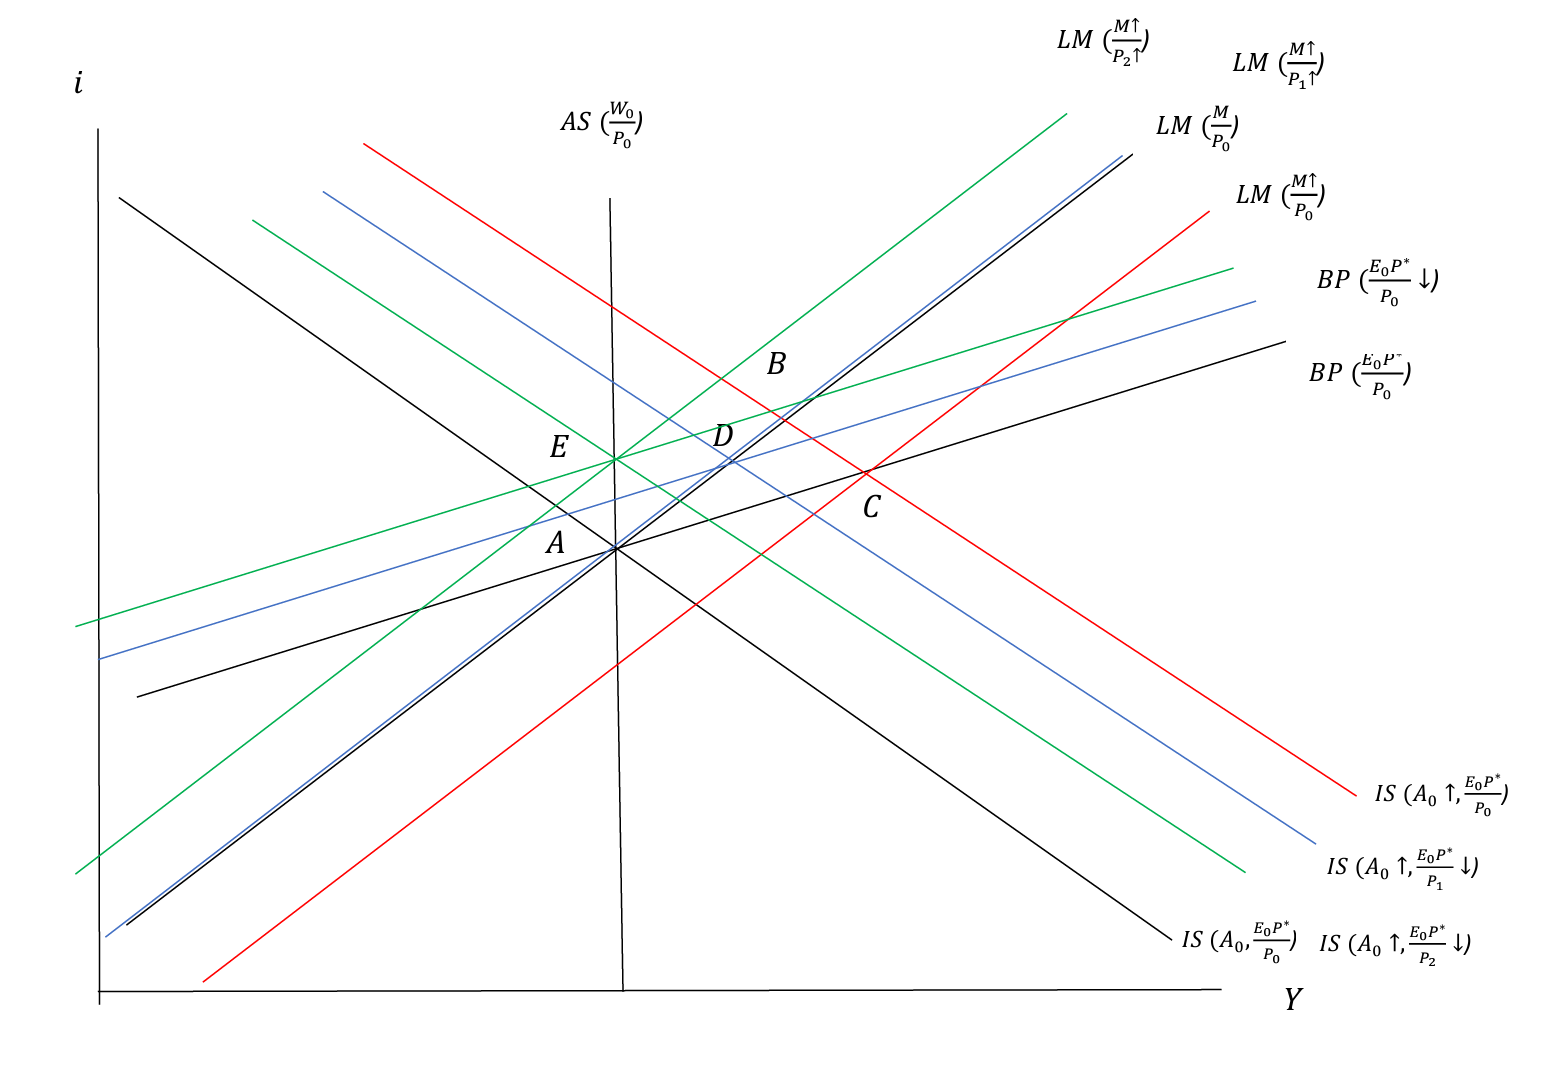
\includegraphics[width=\textwidth]{SCR-20240703-kthq.png}
    \end{figure}
    
    
\end{frame}

\section{סדר פעולות לפתרון בשע''ח נייד}
\begin{frame}[allowframebreaks]
    \frametitle{סדר פעולות לפתרון בשע''ח נייד}
    \begin{block}{שלב $I$}
        סרטוט של מצב המוצא תוך דגש על התייחסות לתנועות הון
        \begin{itemize}
            \item משק סגור לתנועות הון - $ISBP$ עם שיפוע של $IS$ במשק סגור
            \item משק פתוח לתנועות הון מושלמות - $ISBP$ גמישה לחלוטין
            \item משק פתוח לתנועות הון $ISBP$ גמישה יותר מעקומת $IS$
        \end{itemize}
    \end{block}

    \begin{block}{שלב $II$}
        סרטוט של השינוי שחל במשק (טווח מיידי)
        \begin{itemize}
            \item $ISBP$ - $C_0 \uparrow, cT_0 \downarrow , I_0 \uparrow, G_0 \uparrow, TR_0 \downarrow, CF_0 \downarrow, i^{\ *} \uparrow$ \\ הרחבה ימינה ולמעלה
            \item $LM$ - $M_0 \downarrow, M^s \uparrow$ \\ הרחבה ימינה ולמטה
        \end{itemize}
    \end{block}

    \begin{block}{שלב $III$}
        מחירים משתנים, אך עדיין לא חוזרים לתוצר פוטנציאלי. \\
        \begin{tikzpicture}
            % First part: Y > Yp
            \node at (0, 2) {$Y > Y_P$};
            \node at (-1, 0) {$P \uparrow$};
            \draw[->] (-0.5, 0) -- (0.5, 0);
            \node at (1, 0) {$\frac{M}{P} \downarrow$};
            \draw[->] (1.5, 0) -- (2.5, 0);
            \node at (3, 0) {$LM \leftarrow$};
        
            % Second part: Y < Yp
            \node at (6, 2) {$Y < Y_P$};
            \node at (5, 0) {$P \downarrow$};
            \draw[->] (5.5, 0) -- (6.5, 0);
            \node at (7, 0) {$\frac{M}{P} \uparrow$};
            \draw[->] (7.5, 0) -- (8.5, 0);
            \node at (9, 0) {$LM \rightarrow$};
        \end{tikzpicture}
    \end{block}
    
    \begin{block}{שלב $IV$}
        טווח ארוך, מחירים ושכר משתנים וחוזרים לתוצר פוטנציאלי
        \begin{tikzpicture}
            % First part: Y > Yp
            \node at (0, 2) {$Y > Y_P$};
            \node at (-1, 0) {$P \uparrow, W \uparrow$};
            \draw[->] (-0, 0) -- (0.5, 0);
            \node at (1, 0) {$\frac{M}{P} \downarrow$};
            \draw[->] (1.5, 0) -- (2, 0);
            \node at (2.5, 0) {$LM \leftarrow$};
        
            % Second part: Y < Yp
            \node at (6, 2) {$Y < Y_P$};
            \node at (5, 0) {$P \downarrow, W \downarrow$};
            \draw[->] (6, 0) -- (6.5, 0);
            \node at (7, 0) {$\frac{M}{P} \uparrow$};
            \draw[->] (7.5, 0) -- (8, 0);
            \node at (8.5, 0) {$LM \rightarrow$};
        \end{tikzpicture}
    \end{block}


    \begin{figure}[scale=2]
        \centering
        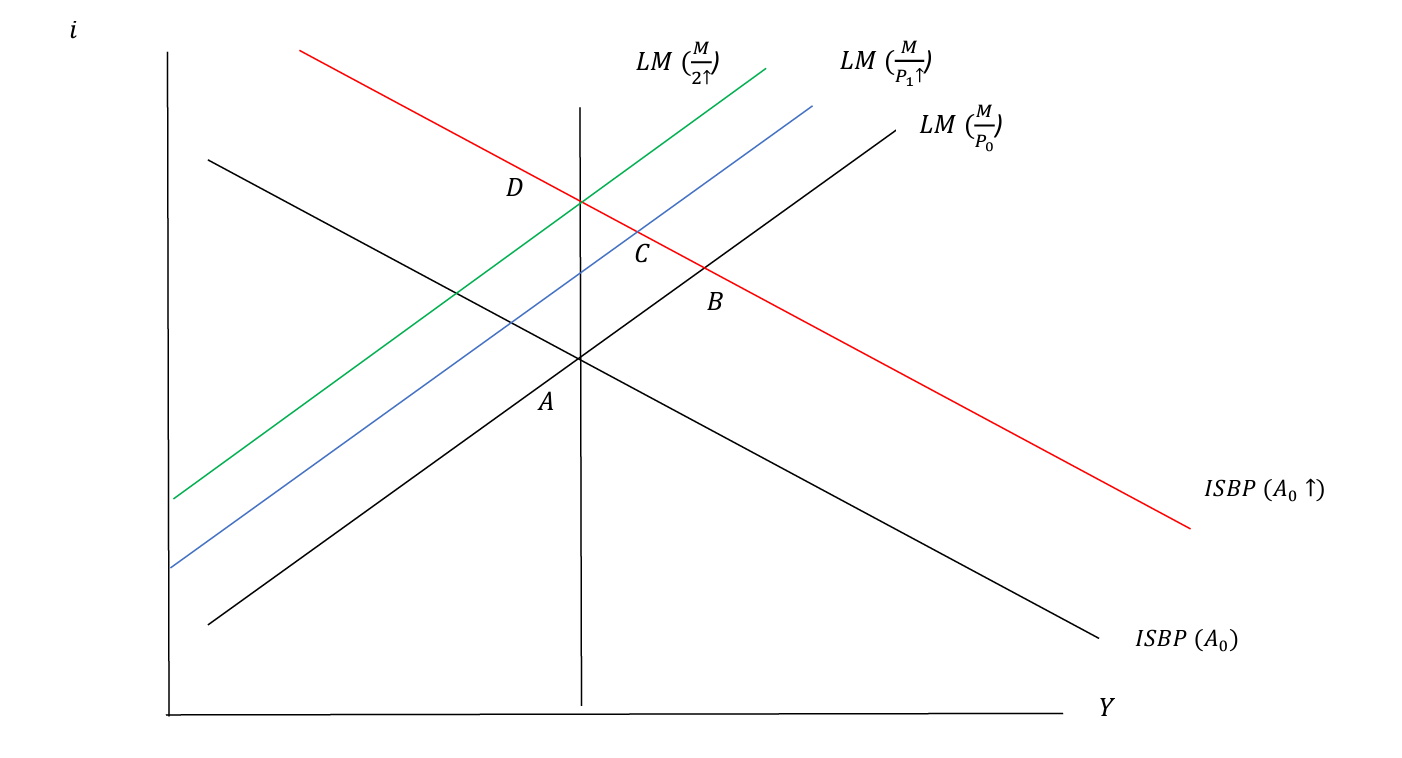
\includegraphics[width=\textwidth]{SCR-20240703-layy.png}
    \end{figure}

\end{frame}

\section{זעזועים פנימיים וחיצוניים}
\begin{frame}
    \frametitle{זעזועים פנימיים וחיצוניים}
    \begin{itemize}
        \item שע''ח נייד מגן על המשק מזעזועים חיצוניים,  $$P^{\ *}\uparrow \implies E \downarrow \implies \overline{\left(\frac{EP^{\, \ast}}{P}\right)}$$ \\   מגן על פני אינפלציה בחו''ל.
        \item שע''ח נייד לא מגן בפני זעזועים פנימיים, $$M_0 \downarrow \implies LM \rightarrow \implies P \uparrow \implies LM\leftarrow$$
        \item שע''ח קבוע לא מגן על המשחק בפני זעזועים חיצוניים, הוא "מייבא אינפלציה מחו''ל". $$P^{\, \ast}\uparrow \implies P \uparrow \implies \overline{\left(\frac{EP^{\, \ast}}{P}\right)}$$
        \item שע''ח קבוע מגן מזעזועים פנימיים $$M_0 \downarrow \implies LM \rightarrow \implies M^s \downarrow \implies LM \leftarrow$$
    \end{itemize}
    

\end{frame}


\section{הטרילמה}
\begin{frame}
    \frametitle{הטרילמה}
    \begin{tikzpicture}
        % Nodes
        \node[rectangle, draw, fill=yellow, text centered, text width=3cm] at (0, 3) {\RTL{תנועות הון חופשיות}};
        \node[rectangle, draw, fill=yellow, text centered, text width=3cm] at (-4, -3) {\RTL{שליטה ב-M וריבית}};
        \node[rectangle, draw, fill=yellow, text centered, text width=3cm] at (4, -3) {\RTL{שליטה בשע"ח}};
    
        % Arrows
        \draw[<->, thick, blue] (-0.5, 2.5) -- (-3.5, -2.5) node[midway, above, sloped] {\RTL{חופשיות הון תנועות עם נייד שע''ח}};
        \draw[<->, thick, blue] (-3.5, -3.5) -- (3.5, -3.5) node[midway, below] {\RTL{עיקורים הון, לתנועות סגור משק}};
        \draw[<->, thick, blue] (3.5, -2.5) -- (0.5, 2.5) node[midway, above, sloped] {\RTL{חופשיות הון תנועות עם קבוע שע''ח}};
    \end{tikzpicture}
    

\end{frame}

\section{איחוד מטבע}
\begin{frame}
    \frametitle{איחוד מטבע}
    \begin{block}{איחוד מטבע}
        
    מספר מדינות בוחרות להשתמש באותו מטבע עם בנק מרכזי אחד שמנפיק את אותו המטבע עבור כל אותן המדינות. המטרה של איחוד זה היא להקל על מעבר של סחורות ולאפשר ניידות של הון ועובדים בין אותן מדינות. בדרך זו נחתכים שערי המרה, פחות בירוקרטיה וקיימת וודאות מלאה לגבי שער החליפין בין אותן מדינות.

\textbf{מתי איחוד מטבע מתאים?}

איחוד מטבע מתאים למדינות אשר קיימים ביניהן מתאם גבוה במחזוריות המאזן הכלכלי. איחוד מטבע כופה על כל אותן המדינות מדיניות מוניטרית אחת אחידה ומדיניות פיסקלית אחידה (ממשלה אחת ומטבע אחד) ולכן באיחוד האירופי המדיניות הפיסקלית איננה אחידה אך המדיניות המוניטרית אחידה (ממשלות רבות ומטבע אחד).
\end{block}
    

\end{frame}
\end{RTL}
\end{document}